\subsection{Finite fields}

A Finite Field $\F_{p^m}$ (also known as Galois Field $GF(p^m)$) is an abstract mathematical structure composed of a set of elements and two operators:

\[
\F_{p^m} = (\{A_0, A_1, A_2, ... A_{p^m-1}\}, +, \cdot)
\]

\begin{itemize}
\item $\F_{p^m}$: A finite field of size $p^m$, where:
    \begin{itemize}
    \item $p$: the \emph{field characteristic}, $p \in \mathbb{P}$ (i.e. must be a prime number);
    \item $m$: the \emph{extension size} $m \geq 1, m \in \mathbb{N}$;
    \end{itemize}
\item $\{A_0, A_1, A_2, ... A_{p^m-1}\}$: A set of $p^m$ \emph{field elements}. In this work we use the names $A$, $B$ and $C$ to refer to arbitrary members of this set.
\item $+, \cdot$~: Addition and multiplication operators, where:
    \begin{itemize}
    \item they are binary operators that operate field elements, $+, \cdot : (\F_{p^m} \times \F_{p^m}) \mapsto \F_{p^m}$;
    \item there are two elements labeled $0$ and $1$ that behave as the additive and multiplicative identities, $0 \neq 1$, such that $\forall A (A + 0 = A~\wedge~A \cdot 1 = A)$;
    \item both operations commute (i.e. $A + B = B + A$ and $A \cdot B = B \cdot A$) and associate (i.e. $(A + B) + C = A + (B + C)$ and $(A \cdot B) \cdot C = A \cdot (B \cdot C)$);
    \item every element has an additive and a multiplicative inverse, also in the field (i.e. there are elements $-A$ and $A^{-1}$ such that $A + -A = 0$ and $A \cdot A^{-1} = 1$);
    \item except the multiplicative identity $0$, which has no multiplicative inverse (i.e. $0^{-1}$ is undefined);
    \item $\underbrace{A + A + A + ... + A}_{\text{$p$ (characteristic) times}} = 0$;
    \end{itemize}
\end{itemize}

All fields of the same size are isomorphic, and therefore a field can be uniquely identified by its size.

There are many ways to construct a field, with modular arithmetic being a common one.
Finite fields are commonly constructed using integer or polynomial modular arithmetic. For example

$$GF(p^m) = (\underbrace{C}_{p^m~\text{elementos}}, \overbrace{+}^{\text{soma}}, \underbrace{\cdot}_{\text{multiplicação}})$$

\begin{gather*}
a, b, c, 0, 1 \in GF(p^m) \\
\\
a + 0 = 0 + a = a \\
a \cdot 0 = 0 \cdot a = 0 \\
a \cdot 1 = 1 \cdot a = a \\
a \cdot a^{-1} = a^{-1} \cdot a = 1 \\
a + (b + c) = (a + b) + c \\
a \cdot (b \cdot c) = (a \cdot b) \cdot c \\
\underbrace{a + a + ... + a}_{p~\text{vezes}} = 0
\end{gather*}

\begin{gather*}
GF(p)\\
5 \cdot 4 \equiv 7 \mod 13 \\
\\
GF(p^m): GF(p^m)[x]/f(x)\\
a = \sum_{i=0}^{m-1} a_i x^i \\
a \in GF(p^m), a_i \in GF(p) \\
\end{gather*}


Representação em bits:
$$[d_{m-1}, d_{m-2}, ..., d_2, d_1, d_0]$$

Representação em palavras:

\begin{figure}[htb]
  \centering
  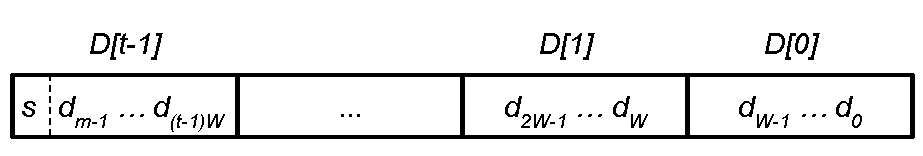
\includegraphics[width = .55\columnwidth]{figures/element-word.pdf}
\end{figure}

\begin{gather*}
a \cdot b = c \equiv d \mod (x^m + x^a + 1) \\
\\
\texttt{reduce}([c_{2m-2}, ..., c_2, c_1, c_0], m, a) \rightarrow [d_{m-1}, ..., d_2, d_1, d_0]
\end{gather*}

\begin{gather*}
x^{m+n} \equiv x^{a+n} + x^n \mod (x^m + x^a + 1)
\end{gather*}

\begin{gather*}
k = \left \lfloor \frac{m-2}{m-a} \right \rfloor + 1 \\
\\
f(x) = x^m + x^{m/2} + 1
\end{gather*}


Introduction

$$ A(x) = \sum_{0}^{m-1} a_i x^i = a_{m-1} x^{m-1} + \ldots + a_1 x + a_0 $$

$$ B(x) = \sum_{0}^{m-1} b_i x^i = b_{m-1} x^{m-1} + \ldots + b_1 x + b_0 $$

$$ a_i, b_i \in GF(2) $$

$$ A \cdot B \pmod{f} $$

Representation

$$ A = (a_0, a_1, \ldots, a_{m-1}) $$

$$ B = (b_0, b_1, \ldots, b_{m-1}) $$

$$ a_i, b_i \in \{0, 1\} $$

$$ a_i + b_i \rightarrow a_i \oplus b_i $$


Reduction

$$ C = (c_0, c_1, \ldots, c_{d}) \mod f,~d \geq m $$


$$ \overbrace{x^{d-m} f(x)}^{\deg d} \equiv 0 \pmod{f(x)}$$

$$ \underbrace{C(x)}_{\deg d} \equiv \underbrace{C(x) + x^{d-m} f(x)}_{\deg~<~d} \pmod{f(x)}$$


$$ C(x) \leftarrow C(x) + \underbrace{c_i}_{\mathclap{\text{avoid conditionals}}} x^{i-m} f(x),~\text{for}~i \in \{d, d-1, \ldots, m\} $$



Example: $C(x) = x^{10}$, $f(x) = x^7 + x^4 + 1$

\begin{align*}
C &= (0, 0, 0, 0, 0, 0, 0, 0, 0, 0, 1)  \\
f &= (1, 0, 0, 0, 1, 0, 0, 1)
\end{align*}


Example: $C(x) = x^{10}$, $f(x) = x^7 + x^4 + 1$

$$ i = 10 $$

$$ C(x) \leftarrow C(x) + c_{10} x^{10-7} f(x)$$

\begin{align*}
C = 00000000001 \\
       10001001 \\
\cline{1-2}
    00010001000
\end{align*}


Example: $C(x) = x^{10}$, $f(x) = x^7 + x^4 + 1$

$$ i = 7 $$

$$ C(x) \leftarrow C(x) + c_{7} x^{7-7} f(x)$$

\begin{align*}
C = 00010001 \\
    10001001 \\
\cline{1-2}
    10011000
\end{align*}


Example: $C(x) = x^{10}$, $f(x) = x^7 + x^4 + 1$

\vspace{2em}

$$ 10011000 \rightarrow x^4 + x^3 + 1 $$

$$ C(x) \mod f(x) =  x^4 + x^3 + 1 $$


$(d-m+1)$ iterations \\
\vspace{1em}
$w_f - 1$ XOR operations per iteration


$$ C(x) \leftarrow C(x) + c_i x^{i-m} f(x),~\text{for}~i \in \{d, d-1, \ldots, m\} $$


Squaring


\begin{align*}
A(x)^2 &= (a_{m-1} x^{m-1} + \ldots + a_1 x + a_0)^2 & \pmod{f(x)} \\
       &= (a_{m-1} x^{m-1})^2 + \ldots + (a_1 x)^2 + (a_0)^2 & \pmod{f(x)} \\
\end{align*}


$$ 0^2 = 0,~1^2 = 1 $$
$$ (a_i)^2 = a_i $$


$$ A(x)^2 = \sum_0^{m-1} a_i x^{2i} \pmod{f(x)} $$


$$ \text{Let}~C = A^2 = \underbrace{(a_0, 0, a_1, 0, \ldots, 0, a_{m-1})}_{m-1 ~\text{guaranteed zeroes}} \pmod{f} $$

$$ C(x) \leftarrow C(x) + c_i x^{i-m} f(x),~\text{for}~i \in \{2m-2, 2m-3, \ldots, m\} $$


$ C = (a_0, 0, a_1, 0, \ldots, 0, a_{m-1}) $

\vspace{1em}

$C[i-m+e] \leftarrow \underbrace{C[i-m+e]}_{\mathclap{\text{case 2}}} \oplus \overbrace{C[i]}^{\mathclap{\text{case 1}}}$

\vspace{1em}

\begin{itemize}
    \item<2-> \textbf{Case 1}: $i$ odd, $C[i]$ not modified
    \item<3-> \textbf{Case 2}: $i-m+e$ odd, $C[i-m+e]$ not modified
    \item<4-> \textbf{Case 3}: normal operation
\end{itemize}


\begin{description}

\item[$m, a$] First non-zero powers of the divisor polynomial, $x^m+x^a+1$.

\item[reduction steps] Number of textbook-division iterations required to reduce the dividend's degree below $m$.

\item[binary field] A field $GF(2)$, implementing with modular addition ($1+1=0$).

\item[binary polynomial] A polynomial where all coefficients are elements of a binary field.

\item[trinomial] A polynomial with exactly three non-zero coefficients and usually in the form $x^m+x^a+1$.

\item[weight (of a polynomial)] Hamming weight of a polynomial, defined as the number of non-zero coefficients.

\item[depth (of an algorithm)] Length of the critical path of the hardware circuit if the algorithm is implemented with XOR gates.

\end{description}